This chapter walks through the chosen technologies, shows the architecture, frames the implementation effort, and explains the decisions taken while working on this thesis. First we will introduce the different technologies and how they play together. Second we will shortly define the frames of reference and the architecture of the implementation. Then the particle filter implementation will be explained in detail, followed by the filter routine and its parameters. Afterwards a few intermediate steps and solved issues that should arise while working on this thesis are discussed. Finally the platform implementation for Android and the effort made on visualization is described.

In order to design, implement and evaluate an online hard iron calibration, two different approaches were taken into consideration. Approach \textit{One}: using existing tools to collect the required sensor data and to process and evaluate it offline. Approach \textit{Two}: designing a system from scratch that collects, processes and visualizes sensor data in real time. Since the outcome of this thesis should be an online algorithm and it seemed to be more target-oriented, the prototyping was created with the paradigm of approach \textit{Two}. Moreover, the orientation estimation (see Section \ref{sec:ori_est}) required qualitative evaluation which was preferable in the online scenario because of the immediate response in the visualization. Approach \textit{One} was later used for the quantitative evaluation of the hard iron calibration.

\section{Technology}

The major criteria for the choice of technology was \textit{platform independence} and \textit{real-time processing}. Platform independence because we are targeting two different mobile platforms with Android and iOS and the need of an evaluation framework that runs on a desktop environment like Ubuntu. Since our calibration should be online, real-time processing is necessary and therefore a critical performance limit is attached to our problem: When one second of real-time has passed we have to process at least one second of input data.

Visualization was planned for prototyping and evaluation purposes. Similar to our calibration algorithm, the visualization was planned to be platform independent with the benefit of displaying it on the smartphone and on the desktop with the same implementation. The first attempt was to use OpenGL from C++ but that introduced a lot of overhead to the implementation. Since all target platforms have an HTML5 compatible browser, the second and final attempt was to use JavaScript for that purpose. To communicate with C++ in real-time, WebSocket was used to exchange Protocol Buffers (see Subsection \ref{sec:protobuf}).

The target platform for the demo application was chosen to be Android. It was developed in Java, responsible for reading the sensors and providing a small user interface.

Table \ref{tbl:code_lines} gives a quick overview about the chosen technologies and the implementation effort by lines of code.

\begin{table}[h]
    \centering
    \begin{tabular}{ | l | r | }
    \hline
    \textbf{Language} & \textbf{Total lines of code} \\ \hline
    C++               & 3092 \\ \hline
    Java              &  366 \\ \hline
    JavaScript        &  450 \\ \hline
    Python            &  179 \\ \hline
    Protocol Buffers  &   55 \\ \hline
    CMake             &  203 \\ \hline
    \end{tabular}
    \caption{Total lines of code by language written for this thesis.}
    \label{tbl:code_lines}
\end{table}

\subsection{C++}

The programming language that was used the most in this project is C++ for various reasons. C++ is platform independent and can reach major smartphone platforms like Android and iOS. Performance was critical for the implementation which is a major purpose of C++. Since C++11 there is a sufficient standard library for common data structures, random variables and common algorithms. Besides that, C++ is a modern programming language with multiple paradigms for example it is object-oriented and generic.

Along with C++ multiple tools, frameworks, and libraries were used which are listed and briefly described below.

\begin{itemize}
  \item \textbf{boost} is a popular C++ library that comes in handy where the standard library is missing functionality. This thesis only depends on \textbf{boost asio} for networking and \textbf{boost beast} for HTTP and WebSocket.
  \item \textbf{Eigen} is a rich library for linear algebra and comes with implementations for matrices, vector, and quaternions.
  \item \textbf{gtest} is a unit test framework from Google and was used to write small self-contained (unit) test cases.
  \item \textbf{CMake} was used as dependency management and build system.
\end{itemize}

\subsection{Android}

Android is a mobile operating system based on a modified version of the Linux kernel and other open source software. It was primarily designed for mobile devices with touchscreen such as smartphones and tablets. Android is developed by a consortium of developers known as the Open Handset Alliance and commercially sponsored by Google. It was unveiled in November 2007, with the first commercial Android device launched in September 2008.

Android has been the best-selling \gls{os} worldwide on smartphones since 2011 and on tablets since 2013. As of May 2017, it has over two billion monthly active users, which is the largest installation base of any operating system.

Android is one of the target platforms for this thesis. Native applications can be developed with Android Studio in Java or Kotlin. Moreover, C++ can be integrated and called through \gls{jni} for shared library access, enabling low-level functionality and high performance applications.

\subsection{JavaScript}

JavaScript was used to realize platform independent visualization that can be displayed on desktop and mobile devices. In contrast to the original approach via OpenGL it was more straight forward to use with \textbf{plotly}\footnote{High level plotting library for Javascript and Python. \url{https://plotly.com}} and a \textbf{matplotlib}\footnote{High level plotting library for Python. \url{https://matplotlib.org}} background in Python. Moreover, modern browsers come with a WebSocket implementation which reduced the complexity of communication to C++ code.

Along with JavaScript multiple tools, frameworks, and libraries were used which are listed and briefly described below.

\begin{itemize}
  \item \textbf{webpack} is a module bundler. Its main purpose is to bundle JavaScript files for usage in a browser.
  \item \textbf{plotly} is a rich plotting library for JavaScript and Python and was used for visualization purposes.
  \item \textbf{THREE} is a library for linear algebra and comes with implementations for matrices, vector, and quaternions.
\end{itemize}

\subsection{Protocol Buffers}
\label{sec:protobuf}

Protocol Buffers\footnote{\url{https://developers.google.com/protocol-buffers}} (short Protobuf) is Google's language-neutral, platform-neutral, extensible mechanism for serializing structured data. It is useful for programs which communicate over a wire or for storing data. Protocol Buffers involve an interface description language which defines the structure of the data. Additionally it comes with a program that generates source code from that definition. The generated code deals with the encoding and decoding of byte streams which represent the structured data.

The data can be serialized in binary representation which takes up less space compared to a text representation like JSON. Therefore it needs less bandwidth while communicating over network.

\section{Frame of reference}
% quaternion transforms from what to what?
% TODO ref images https://developer.android.com/reference/android/hardware/SensorEvent

An important choice while dealing with sensors that have spatial orientation is the frame of reference. Two frames had to be chosen. A local one for the phone and its sensors and a global one for the user and his environment. The chosen axes for the frames of reference are shown in Figure \ref{fig:frames_of_reference} and align with those defined in the Android sensor SDK. While magnetometer readings are taken in the phone's frame of reference it is important to transform those measurements to the global frame of reference since there the magnetic field is expected to be constant in close proximity.\cite{android_sdk_sensorevent}

The transformation between those two frames is estimated by the orientation filter which forms an \gls{imu} based on the accelerometer and gyroscope. While the accelerometer provides information about two orientation angles, the gyroscope can be used to make the estimate more reliable. Additionally, with the gyroscope we can give an relative estimate about the horizontal orientation between two points in time. That angle will drift due to measurement errors which accumulate over time essentially generating a random walk.

In this thesis an algorithm designed by Madgwick was used to estimate the orientation of the phone. See Section \ref{sec:ori_est} for further details.

\begin{figure}[hbt!]
    \centering
    \begin{subfigure}{0.4\textwidth}
        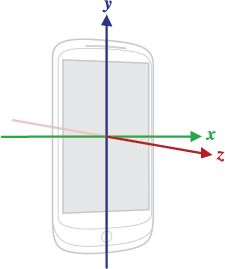
\includegraphics[height=1.0\linewidth]{figures/coords_phone.png}
        \caption{}
    \end{subfigure}
    \begin{subfigure}{0.4\textwidth}
        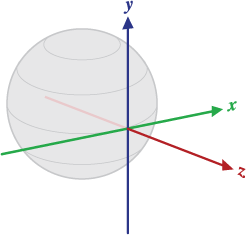
\includegraphics[height=1.0\linewidth]{figures/coords_global.png}
        \caption{}
    \end{subfigure}
    \caption{Chosen frames of reference. With (a) the \textit{local frame of reference} or \textit{device coordinates} and (b) the \textit{global frame of reference} or \textit{world coordinates}. Images gracefully taken from Google's Android SDK documentation.\cite{android_sdk_sensorevent}}
    \label{fig:frames_of_reference}
\end{figure}

\section{Software architecture}

Since the implementation was growing fast in complexity, it was important to structure the project into logical and modular components. Many thoughts went into code architecture and design decisions which will be shortly discussed here.

The desired architecture had to deal with multiple programming languages and potential concurrency issues. Moreover, algorithms should be modules that only depend on their inputs and generate outputs, which makes it easy to exchange them and test them in a generalized way. Another advantage could be the ability to systematically detect bottle necks.

The various algorithms ended up being pluggable components in a pipelining scheme. Sensor and filtered data is passed through pipes from processing entity to processing entity. These processing entities were called nodes. The architecture was applied to the C++ code and the messaging protocol defined with Protocol Buffers. It was also applied in JavaScript but in a more simplified fashion. On Android, Java was used to call \gls{jni} wrapper functions to C++ and therefore did not require any particular architecture.

The overall architecture and different modules are shown in Figure \ref{fig:architecture}.

\begin{figure}[hbt!]
    \centering
    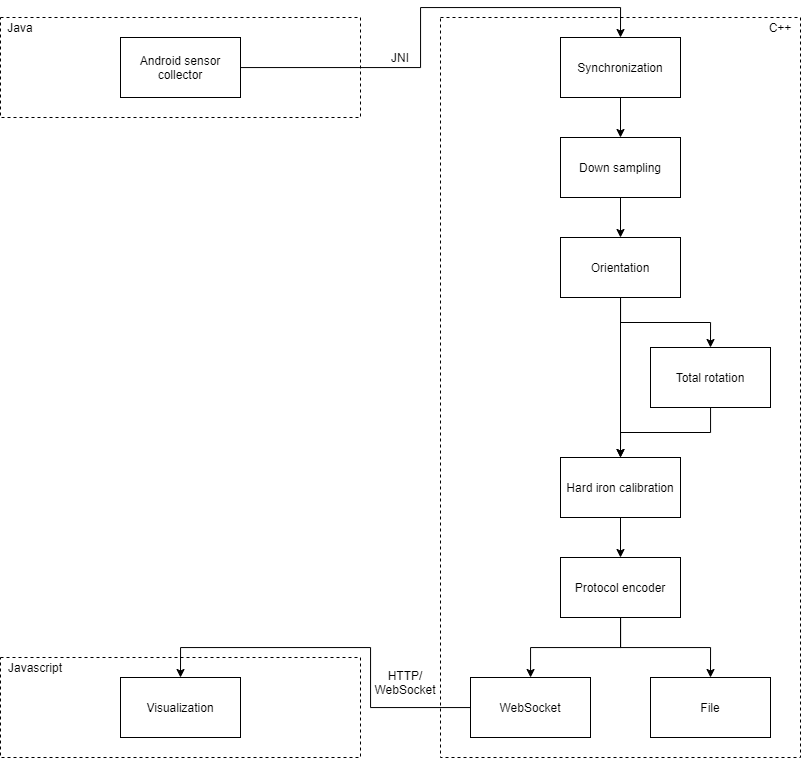
\includegraphics[width=1.0\textwidth]{figures/architecture.png}
    \caption{Illustration of the software architecture grouped by programming language.}
    \label{fig:architecture}
\end{figure}

\section{Particle filter}
\label{sec:impl_pf}
% TODO refer to particle filter section?

In the following subsections we will walk through the different components of the particle filter. First, potential numerical issues with likelihoods are discussed. Second, the representation of a single particle in the filter is presented. Afterwards, the initialization, propagation, update, and resampling steps are discussed. Finally, we will see how the hidden states are estimated.

The bootstrap particle filter\cite{Doucet2011}\cite{Kuensch2013} was chosen as a template for the following implementation.

Initially, the particle filter was designed to model the complete decomposition given in Equation \ref{eq:decomposition} and \ref{eq:decomposition_earth_env}. Since $\bm{B}_\text{earth}$ and $\bm{B}_\text{env}$ transform in the same way under rotation of the device and we do not have a model for $\bm{B}_\text{env}$ this approach failed. The particle filter was further simplified to only decompose Equation \ref{eq:decomposition}.

\subsection{Likelihood}

In Bayesian statistics, likelihood is the key to model the update from a prior to a posterior distribution. Since we do this numerically, we have to be careful with the numerical limitations of the underlying machine. We expect single-precision floating-points as IEEE 754-1985 with the following properties: 1 sign bit, 8 exponent bits, 23 significant precision bits. This leads to an exponent int the range $[-126,127]$. Since likelihood arithmetic involves multiplications with very small numbers we have to use the log likelihood instead.

To calculate the weights from the log likelihood we used the largest log likelihood involved and subtract it from all log likelihoods. This is possible because the weights are invariant under scalar multiplication as a relative measure and can be renormalized if necessary. Additionally this technique maps the weights to numbers in the range $[0,1]$.

\subsection{One particle}

One particle represents the state of one realization of the hard iron calibration. Table \ref{tbl:one_particle} summarizes the properties of one particle. The calibration can be parameterized with a three dimensional vector representing the offset of the measurement from the true value. Another vector keeps the estimated external field, denoted by $\bm{B} = \bm{B}_\text{measure} - \bm{B}_\text{phone}$ with $\bm{B}_\text{phone}$ as the hard iron offset. The external field will later be compared to the next estimate to check for consistency. We also store the \textsc{logLikelihood} later also denoted by $\ell$ and the \textsc{weight} later also denoted by $\mathcal{W}$. They are related to each other but it is handy to keep them separate. Moreover, this might have performance advantages since we do not need to convert between them all the time.

\begin{table}[h]
    \centering
    \begin{tabular}{ | l | p{10cm} | }
    \hline
    \textbf{Field}             & \textbf{Description} \\ \hline
    \textsc{hardIron}          & The hard iron offset represented by this particle. \\ \hline
    \textsc{external}          & The external magnetic field $\bm{B}$ consistent with the last measurement. \\ \hline
    \textsc{logLikelihood}     & Logarithm of the likelihood $\ell$ of this particle. \\ \hline
    \textsc{weight}            & The weight $\mathcal{W}$ of this particle which describes how likely this realization is. It is a relative measure to the total weight among all particles. \\ \hline
    \end{tabular}
    \caption{Description of the properties of one particle.}
    \label{tbl:one_particle}
\end{table}

\subsection{Initialization}

The particle filter has to be initialized with a prior distribution for the hard iron calibration. Pseudocode for the initialization step is given in Algorithm \ref{alg:pf_init}. Without making any further assumptions, a Gaussian distribution $\text{N}(0, \sigma^2)$ was chosen to sample each component of the hard iron vector. In order to enforce the constraint $\bm{B}_\text{measure} = \bm{B}_\text{phone} + \bm{B}$ (see Equation \ref{eq:decomposition}), we need an initial magnetometer observation $\bm{B}_\text{measure}$.

Two potential improvements to the initialization were identified. First, if the device was calibrated in the past, we could choose that as the center of our distribution or mix it with the one at the origin. Second, the current calibration of the operating system might also be a reasonable starting point of our calibration.

\begin{algorithm}[h]
	\KwIn{population size $N$, hard iron variance $\sigma^2$, magnetic field measurement $\bm{B}_\text{measure}$, orientation $\bm{q}$}
	\KwOut{initialized and populated particle filter $P$}
	$P \leftarrow$ \textsc{allocateParticles}($N$)\\
	\ForEach{particle in $P$}{
		$\bm{B}_\text{phone} \leftarrow$ \textsc{gaussianDrawThree}($0$, $\sigma^2$)\\
		\smallskip
		$\bm{B} \leftarrow q \times (\bm{B}_\text{measure} - \bm{B}_\text{phone})$\\
		\smallskip
		$\ell \leftarrow -\log{N}$\\
		\smallskip
		$\mathcal{W} \leftarrow \frac{1}{N}$\\
	}
	\Return{$P$}
	\caption{Initialization of the particle filter as pseudocode.}
	\label{alg:pf_init}
\end{algorithm}

\subsection{Prediction}

In order to predict future states of our particles we have to apply the state transition. Pseudocode for the propagation step can be found in Algorithm \ref{alg:pf_prop}. Since we do not have a physical model for the time evolution of the hard iron effect, the idea was to apply a random walk for each particle. This approach allows the particle filter to do recalibration over time.

\begin{algorithm}[h]
	\KwIn{population $P$, time passed $t$, hard iron variance drift rate $\sigma^2$}
	\KwOut{population $P$}
	\ForEach{particle in $P$}{
		$\bm{B}_\text{phone} \leftarrow \bm{B}_\text{phone}$ + \textsc{gaussianDrawThree}($0$, $t * \sigma^2$)\\
	}
	\Return{$P$}
	\caption{Prediction step of the particle filter as pseudocode.}
	\label{alg:pf_prop}
\end{algorithm}

\subsection{Update}

We update our particle filter by feeding it with new observations from the magnetometer and new estimates of the orientation filter (see Section \ref{sec:ori_est}). Pseudocode for the update step is given in Algorithm \ref{alg:pf_update}. We predict the measurement of the magnetic field $\bm{B}_\text{measure}$ by transforming the previous estimate of the external field $\bm{B}$ into the local frame of reference and adding the hard iron vector $\bm{B}_\text{phone}$. Based on that prediction $\hat{\bm{B}}_\text{measure}$ and the measurement $\bm{B}_\text{measure}$, a likelihood can be calculated. That likelihood was modeled by a Gaussian distribution $N(0, \sigma^2)$. $\sigma^2$ can be used to parameterize the noise of the sensor and the variation of the magnetic field between two different points in space.

\begin{algorithm}[hbt!]
	\KwIn{population $P$, magnetic field measurement $\bm{B}_\text{measure}$, orientation $\bm{q}$, prediction variance $\sigma^2$}
	\KwOut{population $P$}
	\ForEach{particle in $P$}{
	    $\hat{\bm{B}}_\text{measure} \leftarrow \bm{B}_\text{phone} + \bm{q}^{-1} \times \bm{B}$\\
	    $\ell \leftarrow \ell +$ \textsc{gaussianLogPDF}($\hat{\bm{B}}_\text{measure}$, $\bm{B}_\text{measure}$, $\sigma^2$)\\
	    $\bm{B} \leftarrow \bm{q} \times (\bm{B}_\text{measure} - \bm{B}_\text{phone})$\\
	}
	\Return{$P$}
	\caption{Update step of the particle filter as pseudocode.}
	\label{alg:pf_update}
\end{algorithm}

\subsection{Resampling}
% TODO refer to particle filter section?

The resampling step is the most important part of the particle filter. Without it the likelihood would converge to zero and the variance of the weights would only increase. The idea is to remove unlikely states and replace them with more likely ones. The chosen algorithm, called multinomial resampling\cite{Doucet2011}\cite{parallel_resampling}, is a common resampling algorithm with a time complexity of $\mathcal{O}(n \ln{n})$ and memory complexity of $\mathcal{O}(n)$.\cite{particle_resample}

Pseudocode for the resampling step is given in Algorithm \ref{alg:pf_resampling}. First we calculate the weight of each particle $\mathcal{W}$ by its likelihood $\ell$. Then we accumulate these weights into an array of partial sums $w_i$. Now we can draw uniformly distributed samples $x$ from the range $0$ to total weight $\mathcal{W}_{sum}$ and lookup the lower bound elements in the array. Thereby we get the indices $i$ of the particles we are going to sample from. We copy the state of those particles $P_{in}^{i}$ into a second array and afterwards exchange it with the previous array of particles (double buffering).

Since the propagation step applies a random walk to the hard iron offset, we do not have to worry about state degeneracy.

\begin{algorithm}[h]
	\KwIn{population $P_{in}$, population size $n$}
	\KwOut{population $P_{out}$}
	$\ell_{max} \leftarrow \textsc{max}(\ell)$\\
	$\mathcal{W}_{sum} \leftarrow 0$\\
	$w \leftarrow$ \textsc{allocateFloats}($n$)\\
	\ForEach{$p$ in $P_{in}$}{
	    $\mathcal{W} \leftarrow e^{\ell - \ell_{max}}$\\
	    $\mathcal{W}_{sum} \leftarrow \mathcal{W}_{sum} + \mathcal{W}$\\
	    $w_i \leftarrow \mathcal{W}_{sum}$\\
	}
	\ForEach{$p$ in $P_{out}$}{
	    $x \leftarrow$ \textsc{random}($0$, $\mathcal{W}_{sum}$)\\
	    $i \leftarrow$ \textsc{lowerBounds}($w$, $x$)\\
	    $p \leftarrow P_{in}^{i}$\\
	}
	\Return{$P_{out}$}
	\caption{Resampling step of the particle filter as pseudocode.}
	\label{alg:pf_resampling}
\end{algorithm}

\subsection{Estimation}

In the estimation step we want to measure the hidden state of our system. The state of the particle filter is represented by its population, the particles, and their states and weights.

Pseudocode for the estimation step is given in Algorithm \ref{alg:pf_estimate}. In order to get an estimate of the hard iron vector and its error, a weighted average and weighted covariance matrix is calculated from the population of the filter. The covariance matrix can later be used to quantify the convergence of the filter.

\begin{algorithm}[h]
	\KwIn{population $P$}
	\KwOut{hard iron vector $\bm{\hat{B}}_{phone}$, hard iron covariance $\bm{\hat{\Sigma}}_{phone}$, external magnetic field vector $\bm{\hat{B}}$, external magnetic field covariance $\bm{\hat{\Sigma}}$}
    $\bm{\hat{B}}_{phone} \leftarrow$ \textsc{weightedAverage}($P$, $\mathcal{W}$, $\bm{B}_\text{phone}$)\\
    $\bm{\hat{\Sigma}}_{phone} \leftarrow$ \textsc{weightedCovariance}($P$, $\mathcal{W}$, $\bm{B}_\text{phone}$)\\
    $\bm{\hat{B}} \leftarrow$ \textsc{weightedAverage}($P$, $\mathcal{W}$, $\bm{B}$)\\
    $\bm{\hat{\Sigma}} \leftarrow$ \textsc{weightedCovariance}($P$, $\mathcal{W}$, $\bm{B}$)\\
	\Return{$\bm{\hat{B}}_\text{phone}$, $\bm{\hat{\Sigma}}_\text{phone}$, $\bm{\hat{B}}$, $\bm{\hat{\Sigma}}$}
	\caption{Estimation step of the particle filter as pseudocode.}
	\label{alg:pf_estimate}
\end{algorithm}

\section{Filter routine}

Our filter routine for the hard iron calibration is a combination of all the steps described in Section \ref{sec:impl_pf}. The parameters of the filter are summarized in Table \ref{tbl:impl_params}.

\begin{table}[h]
    \centering
    \begin{tabular}{ | l | p{10cm} | }
    \hline
    \textbf{Parameter}       & \textbf{Description} \\ \hline
    \textsc{seed}                   & Seed for the pseudorandom number generator. \\ \hline
    \textsc{population}             & The total number of particles. \\ \hline
    \textsc{deltaTime}              & The time difference in seconds between two filter iterations. \\ \hline
    \textsc{initialVariance}        & The initial hard iron variance for the initialization procedure in $(\mu T)^2$. \\ \hline
    \textsc{driftRate}              & The hard iron calibration drift rate for the propagation procedure. \\ \hline
    \textsc{predictionVariance}     & The prediction variance for the update procedure in $(\mu T)^2$. \\ \hline
    \textsc{minimalRotation}        & Minimal rotation angle to perform an update in radians. \\ \hline
    \textsc{resamplingRate}         & Relative amount of effective particles to trigger resampling. \\ \hline
    \end{tabular}
    \caption{Parameter description of the filter.}
    \label{tbl:impl_params}
\end{table}

Pseudocode of the filter routine is given in Algorithm \ref{alg:routine}. We initialize the filter with the first observations of the magnetometer and orientation filter. Then we update and propagate based on time passed and newly incoming observations. The filter will only update after significant rotations which is parameterized by \textsc{minimalRotation}. This has the benefit of saving \gls{cpu} consumption and filtering noise of the orientation estimation which could result in biased hard iron estimates. Adaptive resampling (see Equation \ref{eq:pf_effective} in Section \ref{sec:pf_resampling}) is used to reduce noise, might spare \gls{cpu} usage and can be parameterized with \textsc{resamplingRate}.

\begin{algorithm}[h]
	\KwIn{magnetic field measurement $\bm{B}_\text{measure}$, orientation $\bm{q}$}
	\KwOut{calibrated magnetic field $\bm{\hat{B}}$, calibrated magnetic field covariance $\bm{\hat{\Sigma}}$}
	\If{\textsc{notInitialized()}}{
	    $P \leftarrow$ \textsc{init}($\bm{B}_\text{measure}$, $\bm{q}$)\\
	    \textsc{estimate}()\\
	}
	\If{\textsc{significantRotation()}}{
	    \textsc{update}($\bm{B}_\text{measure}$, $\bm{q}$)\\
	    $\bm{\hat{B}}_{phone}$, $\bm{\hat{\Sigma}}_{phone}$ $\leftarrow$ \textsc{estimate}()\\
	    \If{\textsc{effectiveParticles()} < \textsc{population} $\times$ \textsc{resamplingRate}}{
	        \textsc{resample}()\\
	    }
	}
	$\bm{\hat{B}} \leftarrow \bm{B}_\text{measure} - \bm{\hat{B}}_{phone}$\\
    $\bm{\hat{\Sigma}} \leftarrow \bm{\hat{\Sigma}}_{phone}$\\
	\Return{$\bm{\hat{B}}$, $\bm{\hat{\Sigma}}$}
	\caption{The filter routine as pseudocode.}
	\label{alg:routine}
\end{algorithm}

\section{Synchronization}
\label{sec:impl_synchro}

Our work targets mobile devices with Android and iOS. Since those are no real-time systems one has to deal with unpredictable latency and concurrency. These effects play a role while receiving data of multiple sensors, possibly through multiple threads. The receiver might observe that some events are out of order. Recursive filters rely on the causal order of the events because the state of the filter evolves with each observation and its timestamp. They cannot include events that are older than the current state. When we combine multiple sensor streams into one result, we have to be careful with potential latency differences given by each stream.

This problem was solved with a synchronization step at the beginning of the pipeline (see Figure \ref{fig:architecture}). Buffers are used to hold all the incoming sensor data until it is guaranteed that all streams reached the same point in time. Additionally, this guarantees that any other component after the synchronization will only receive events in order and does not have to deal with synchronization by itself.

\section{Down sampling}
\label{sec:impl_downsample}

As mentioned in Section \ref{sec:impl_synchro}, we cannot rely on the properties of a real-time system. In case of Android, the requested sampling rate passed to the the sensors \gls{api} is treated as a hint and can differ greatly. Since the orientation estimation (see Section \ref{sec:ori_est}) relies on a constant sampling rate, this problem had to be resolved by implementing a down sampling algorithm. The chosen algorithm was a moving average.

The sampling interval was measured during the evaluation in Section \ref{sec:eval_sensor}.

\section{Orientation estimation}
\label{sec:ori_est}

We saw that our hard iron calibration highly depends on the orientation estimation of the device in Section \ref{sec:impl_pf}. Errors attached to the orientation estimates will directly propagate into errors of the hard iron calibration. Therefore it was crucial to use a well suited algorithm to estimate the orientation with high precision. These algorithms typically use the accelerometer and the gyroscope to form an \gls{imu}.

In our implementation we relied on Madgwick's \gls{imu} algorithm\cite{madgwick} which estimates the orientation by fusing accelerometer and gyroscope. It claims to have low computational effort and higher accuracy than Kalman-based algorithms. The algorithm is illustrated in Figure \ref{fig:madgwick_imu}. The orientation filter has only a single parameter \textsc{beta}, apart from the update interval, which models the reliability proportion between accelerometer and gyroscope measurements.

\begin{figure}[hbt!]
    \centering
    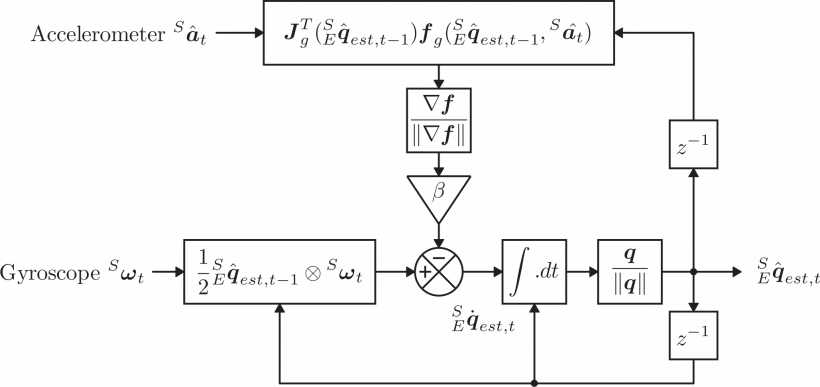
\includegraphics[width=1.0\textwidth]{figures/madgwick_imu.png}
    \caption{Block diagram representation of the orientation estimation algorithm. Image gracefully taken from Madgwick's paper.\cite{madgwick}}
    \label{fig:madgwick_imu}
\end{figure}

Implementations for various programming languages are available online\footnote{\url{https://x-io.co.uk/open-source-imu-and-ahrs-algorithms}}, including an implementation for C. This C implementation was adopted for C++ and slightly modified. One of the modifications was the replacement of the ``fast inverse square-root'' by a more conventional implementation. The ``fast inverse square-root'' was producing biases and the computational performance was not too critical in our case anyway.

With an \gls{imu} based on accelerometer and gyroscope, the x and y-axis in world coordinates (see Figure \ref{fig:frames_of_reference}) will be rotated by an unknown angle around the z-axis. This is due to missing information of the horizontal orientation, which can only be observed by the magnetometer (in case of those three sensors). Moreover, this angle will be drifting due to accumulated errors coming from the gyroscope.

\section{Total rotation}

Since our hard iron calibration can only progress if the device is rotated, we might want to quantify the total rotation and use it instead of time as an axis for our prototyping and evaluation plots. This was achieved by calculating the Euler axis and angle between two orientation estimates and a sum over these angles.

The quaternion $\bm{\Delta q}_i$ that transforms the previous orientation $\bm{q}_{i-1}$ to the current orientation $\bm{q}_i$ can be expressed by the following equation.

\begin{equation}
\label{eq:impl_totalrot_q}
    \bm{q}_i = \bm{\Delta q}_i \times \bm{q}_{i-1} \iff \bm{\Delta q}_i = \bm{q}_i \times \bm{q}_{i-1}^{-1}
\end{equation}

The Euler angle can then be extracted with the extended Euler's formula.

\begin{equation}
\label{eq:impl_totalrot}
    \Delta \omega_i = 2 \arccos{\operatorname{Re}(\bm{\Delta q}_i)}
\end{equation}

With $\operatorname{Re}(\bm{\Delta q}_i)$ as the real component of the quaternion $\bm{\Delta q}_i$.

The summation over $\Delta \omega_i$ is our desired quantity ``total rotation''. This quantity was also used to filter for significant rotations in the filter routine of our hard iron calibration.

\section{Android}

Java was used to develop a small demo application that is able to read sensor data and pass it down to C++ through \gls{jni}. A \textsc{WebView} was used to display the visualization written in JavaScript. The whole life cycle of the application was managed in Java.

The Android sensor \gls{api} offers a high-level interface to read sensor values by registering to a specific sensor type, like accelerometer, providing a sampling rate, and a callback for incoming data. The \gls{api} is presenting calibrated and uncalibrated sensor readings in the same way and is distinguishing between them by different identifiers. \textsc{TYPE\_MAGNETIC\_FIELD} can be used to read the system calibrated magnetic field and \textsc{TYPE\_MAGNETIC\_FIELD\_UNCALIBRATED} for the uncalibrated magnetic field, which is required by this thesis.\cite{android_sdk_sensormanager}

From experience we know that the sensor \gls{api} will not sample the sensors at a constant rate. Since a constant sampling rate is a requirement for the orientation filter, this problem had to be resolved as discussed in Section \ref{sec:impl_downsample}.

A screenshot of the demo application is shown in Figure \ref{fig:app}.

\begin{figure}[hbt!]
    \centering
    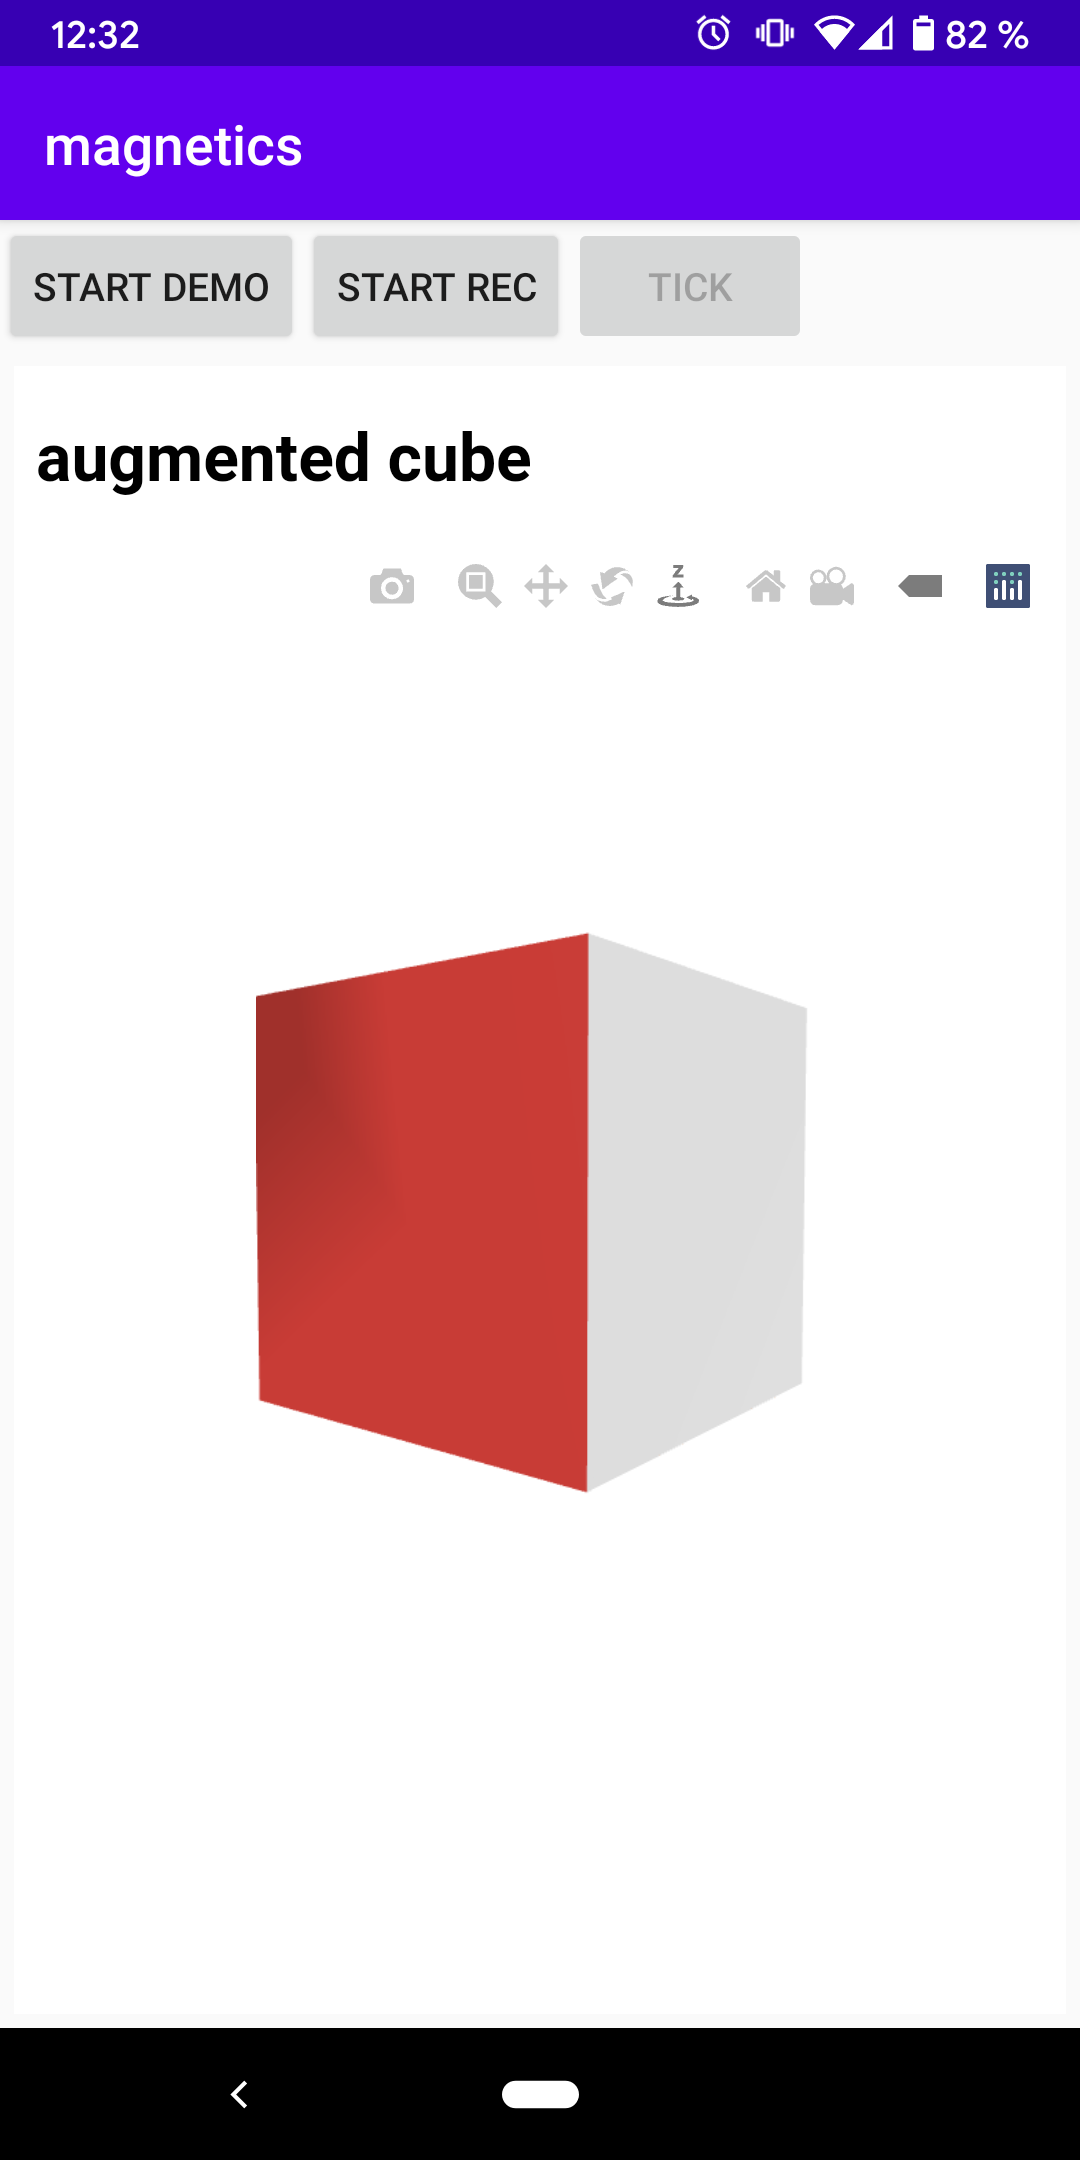
\includegraphics[width=0.4\textwidth]{figures/app.png}
    \caption{Screenshot for the Android demo application.}
    \label{fig:app}
\end{figure}

\section{Visualization}

One goal of the visualization was to make it platform independent and to use the same code for desktop and mobile devices. This was beneficial because the visualization could also be driven by simulated and real-time sensor data.

% TODO dont tell the whole story. just state two options. then why one was preferred over the other
The initial idea was to use OpenGL ES for visualization purposes. Android and common desktop \gls{os} support OpenGL. One visualization idea was a three-dimensional scatter plot for the acquired magnetic field sensor data to build up intuition for the data we are going to filter. This might require to plot thousands of data points in real time. Since OpenGL is executed by the \gls{gpu} there were no performance concerns.

Since implementation progress was rather slow and the effort was growing quickly the desire for an alternative was growing. JavaScript with plotly seemed to be a good solution for platform independence. It also claimed to have good performance with a WebGL backend for 3D plots.

The HTML and JavaScript code was stored as an asset along the demo application and was displayed by a \textsc{WebView} on Android. On the desktop it is sufficient to use any modern browser to run the visualization.
